% Myno — simple architecture diagram with icons.
% Build:  pdflatex architecture.tex
% Self-contained: icons are hand-drawn in TikZ (no font/asset dependencies).
\documentclass[tikz,border=14pt]{standalone}
\usepackage{tikz}
\usetikzlibrary{positioning,arrows.meta,calc}

% Serene Care palette — matches the website (frontend/src/App.jsx, const C)
\definecolor{teal}{HTML}{366366}    % primary
\definecolor{tealC}{HTML}{4F7C7F}   % lighter teal (speech services)
\definecolor{rose}{HTML}{C98A93}    % dusty rose (roseDeep)
\definecolor{mauve}{HTML}{775C5C}   % roseOn
\definecolor{amber}{HTML}{A9772A}   % accent
\definecolor{slate}{HTML}{707979}   % outline / neutral
\definecolor{ink}{HTML}{1B1C1C}     % primary text
\definecolor{inkvar}{HTML}{404849}  % secondary text

% ---------- flat line icons (use `pic actions` so the call's color applies) ----------
\tikzset{
  ic browser/.pic={
    \draw[pic actions, rounded corners=1.2pt] (-.5,-.4) rectangle (.5,.4);
    \draw[pic actions] (-.5,.2) -- (.5,.2);
    \draw[pic actions] (-.4,.3) circle (.035);
    \draw[pic actions] (-.3,.3) circle (.035);
    \draw[pic actions] (-.2,.3) circle (.035);
  },
  ic mic/.pic={
    \draw[pic actions, rounded corners=.13cm] (-.13,0) rectangle (.13,.46);
    \draw[pic actions] (-.27,.12) arc (180:360:.27);
    \draw[pic actions] (0,-.15) -- (0,-.36);
    \draw[pic actions] (-.2,-.36) -- (.2,-.36);
  },
  ic wave/.pic={ % ASR — audio waveform
    \foreach \x/\h in {-.42/.16,-.27/.36,-.12/.24,.03/.42,.18/.2,.33/.32}
      \draw[pic actions, line cap=round] (\x,-\h) -- (\x,\h);
  },
  ic robot/.pic={ % LLM
    \draw[pic actions, rounded corners=3pt] (-.36,-.3) rectangle (.36,.32);
    \draw[pic actions] (0,.32) -- (0,.47);
    \draw[pic actions, fill=white] (0,.5) circle (.045);
    \draw[pic actions, fill=white] (-.17,.02) circle (.07);
    \draw[pic actions, fill=white] (.17,.02) circle (.07);
    \draw[pic actions, line cap=round] (-.14,-.16) -- (.14,-.16);
  },
  ic speaker/.pic={ % TTS
    \draw[pic actions] (-.42,-.16) -- (-.42,.16) -- (-.2,.16) -- (.06,.4) -- (.06,-.4) -- (-.2,-.16) -- cycle;
    \draw[pic actions] (.2,-.2) arc (-50:50:.24);
    \draw[pic actions] (.34,-.32) arc (-48:48:.4);
  },
  ic chart/.pic={ % math insights
    \draw[pic actions] (-.45,.42) -- (-.45,-.36) -- (.46,-.36);
    \foreach \x/\h in {-.32/.2,-.07/.4,.18/.62}
      \draw[pic actions, fill=white] (\x,-.36) rectangle ++(.16,\h);
  },
  ic book/.pic={ % research literature
    \draw[pic actions] (-.42,-.3) -- (-.42,.3) -- (0,.42) -- (0,-.18) -- cycle;
    \draw[pic actions] ( .42,-.3) -- ( .42,.3) -- (0,.42) -- (0,-.18) -- cycle;
  },
  ic db/.pic={ % database cylinder
    \draw[pic actions] (-.3,.32) arc (180:0:.3 and .12);
    \draw[pic actions] (-.3,.32) -- (-.3,-.3) arc (180:360:.3 and .12) -- (.3,.32);
    \draw[pic actions] (-.3,.32) arc (180:360:.3 and .12);
    \draw[pic actions] (-.3,.02) arc (180:360:.3 and .12);
  },
  ic cross/.pic={ % private healthcare
    \draw[pic actions, line cap=round] (0,-.32) -- (0,.32);
    \draw[pic actions, line cap=round] (-.32,0) -- (.32,0);
  },
  ic heart/.pic={ % adjacent conditions
    \draw[pic actions] (0,-.3)
      .. controls (-.5,.06) and (-.26,.42) .. (0,.16)
      .. controls (.26,.42) and (.5,.06) .. (0,-.3);
  },
  ic flask/.pic={ % real-world evidence
    \draw[pic actions] (-.12,.36) -- (-.12,.04) -- (-.36,-.34) -- (.36,-.34) -- (.12,.04) -- (.12,.36);
    \draw[pic actions] (-.2,.36) -- (.2,.36);
    \draw[pic actions] (-.27,-.14) -- (.27,-.14);
  },
  ic pie/.pic={ % population / payer insights
    \draw[pic actions] (0,0) circle (.34);
    \draw[pic actions] (0,0) -- (0,.34);
    \draw[pic actions] (0,0) -- (.31,.14);
  },
}

\tikzset{
  block/.style={rounded corners=7pt, draw=#1, line width=1.1pt, fill=#1!7,
                minimum width=33mm, minimum height=24mm, align=center,
                font=\sffamily, text=ink, inner sep=4pt},
  bizblock/.style={rounded corners=7pt, draw=#1, line width=1pt, dash pattern=on 3pt off 2pt,
                fill=#1!5, minimum width=33mm, minimum height=22mm, align=center,
                font=\sffamily, text=ink, inner sep=4pt},
  cap/.style={font=\sffamily\bfseries\small, text=ink},
  sub/.style={font=\sffamily\scriptsize, text=slate},
  arr/.style={-{Stealth[length=2.6mm]}, line width=1.2pt, draw=slate},
  edgelbl/.style={font=\sffamily\scriptsize, text=slate, fill=white, inner sep=2pt},
}

% place a block + an icon centred in its upper third, with caption + sublabel
\newcommand{\blk}[6]{% (#1 name)(#2 color)(#3 icon)(#4 caption)(#5 sublabel)(#6 at-coord)
  \node[block=#2] (#1) at (#6)
    {\rule{0pt}{11mm}\\[1pt]{\sffamily\bfseries\small\color{ink}#4}%
     \\[1pt]{\sffamily\scriptsize\color{inkvar}#5}};
  \pic[#2, line width=1.1pt] at ($(#1.north)+(0,-6mm)$) {#3};
}

% business-opportunity block (dashed = potential, not built)
\newcommand{\bizblk}[6]{% (#1 name)(#2 color)(#3 icon)(#4 caption)(#5 sublabel)(#6 at-coord)
  \node[bizblock=#2] (#1) at (#6)
    {\rule{0pt}{10mm}\\[1pt]{\sffamily\bfseries\small\color{ink}#4}%
     \\[1pt]{\sffamily\scriptsize\color{inkvar}#5}};
  \pic[#2, line width=1.1pt] at ($(#1.north)+(0,-5.5mm)$) {#3};
}

\begin{document}
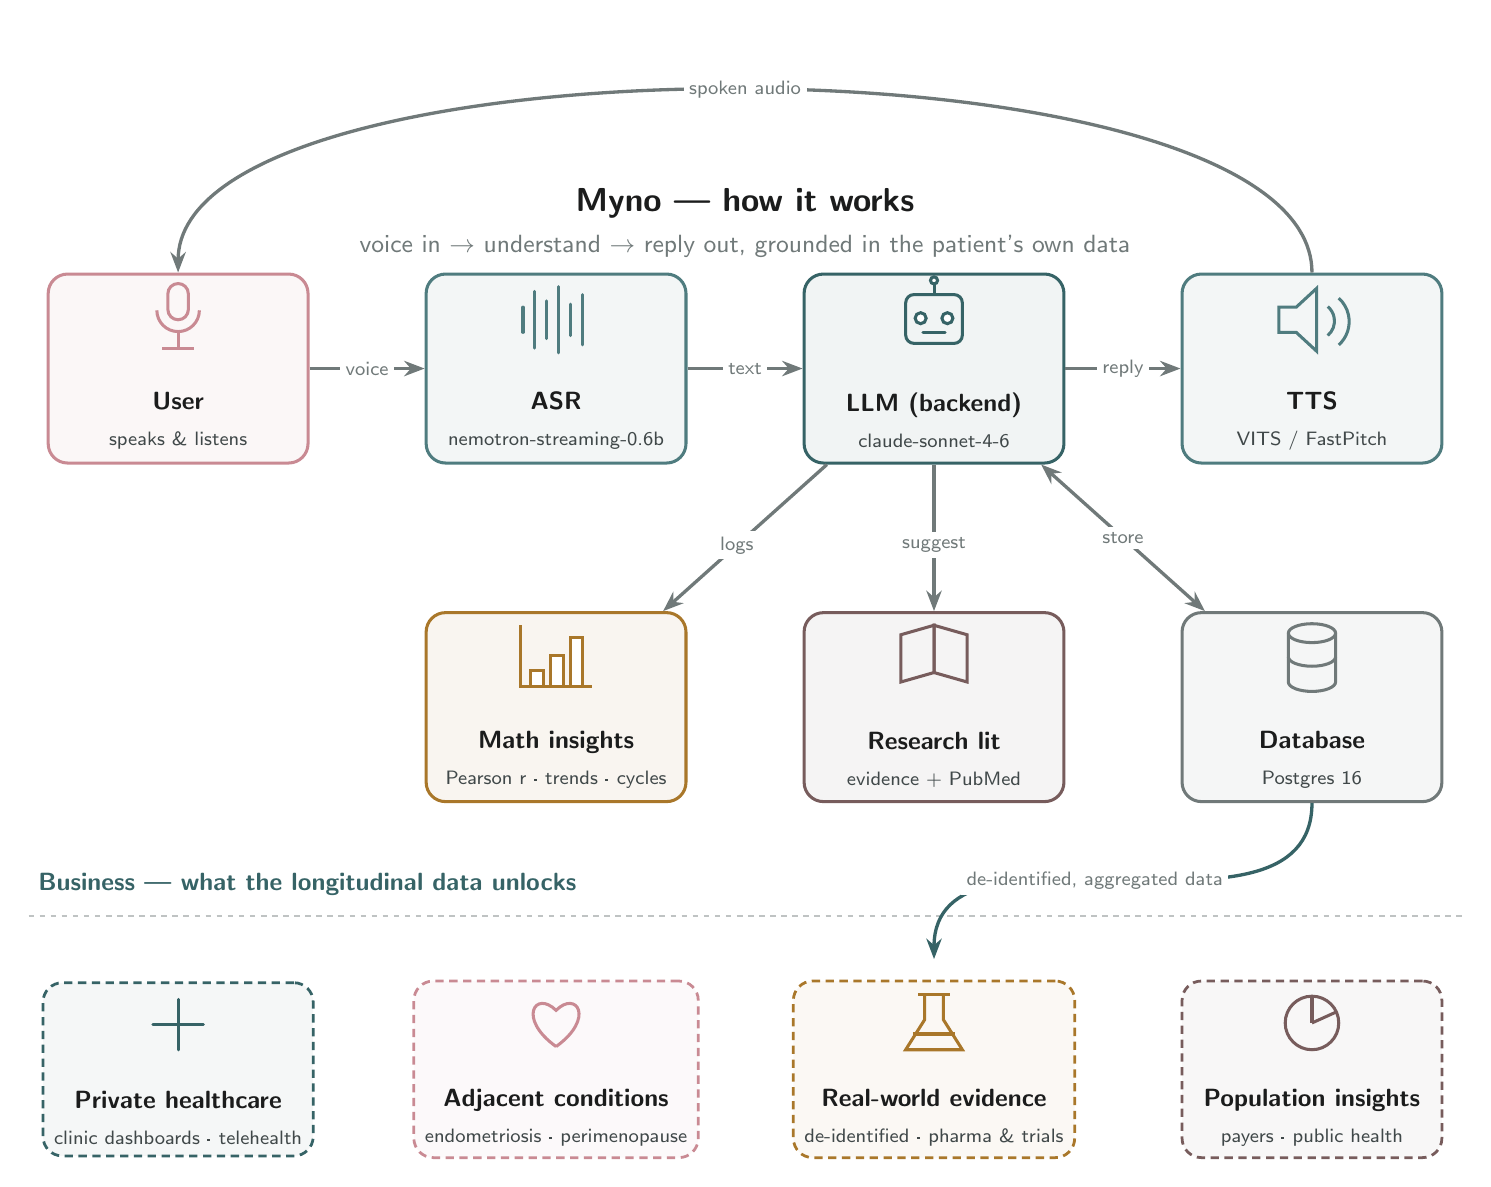
\begin{tikzpicture}[x=1cm,y=1cm]

\node[font=\sffamily\bfseries\large, text=ink] at (7.2,2.1) {Myno — how it works};
\node[font=\sffamily\small, text=slate] at (7.2,1.55)
  {voice in $\to$ understand $\to$ reply out, grounded in the patient's own data};

% ---- main voice loop (left to right) ----
\blk{user}{rose}{ic mic}{User}{speaks \& listens}{0,0}
\blk{asr}{tealC}{ic wave}{ASR}{nemotron-streaming-0.6b}{4.8,0}
\blk{llm}{teal}{ic robot}{LLM (backend)}{claude-sonnet-4-6}{9.6,0}
\blk{tts}{tealC}{ic speaker}{TTS}{VITS / FastPitch}{14.4,0}

% ---- support row: what the backend draws on ----
\blk{math}{amber}{ic chart}{Math insights}{Pearson r \textperiodcentered{} trends \textperiodcentered{} cycles}{4.8,-4.3}
\blk{lit}{mauve}{ic book}{Research lit}{evidence + PubMed}{9.6,-4.3}
\blk{db}{slate}{ic db}{Database}{Postgres 16}{14.4,-4.3}

% ---- voice loop arrows ----
\draw[arr] (user) -- node[edgelbl]{voice} (asr);
\draw[arr] (asr)  -- node[edgelbl]{text} (llm);
\draw[arr] (llm)  -- node[edgelbl]{reply} (tts);
\draw[arr] (tts.north) to[out=90,in=90,looseness=0.55]
      node[edgelbl]{spoken audio} (user.north);

% ---- backend draws on stats / literature / store ----
\draw[arr] (llm) -- node[edgelbl,pos=0.55]{logs} (math);
\draw[arr] (llm) -- node[edgelbl,pos=0.55]{suggest} (lit);
\draw[{Stealth[length=2.6mm]}-{Stealth[length=2.6mm]}, line width=1.2pt, draw=slate]
      (llm) -- node[edgelbl,pos=0.5]{store} (db);

% ===== BUSINESS LAYER — what the longitudinal data unlocks =====
% divider + section title
\draw[draw=slate!45, line width=.6pt, dash pattern=on 2pt off 2pt]
      (-1.9,-6.95) -- (16.3,-6.95);
\node[anchor=west, font=\sffamily\bfseries\small, text=teal] at (-1.9,-6.55)
      {Business — what the longitudinal data unlocks};

% data feeds the opportunities
\draw[arr, draw=teal] (db.south) to[out=-90,in=90]
      node[edgelbl, pos=0.55]{de-identified, aggregated data} (9.6,-7.5);

% opportunity blocks (dashed = potential, not yet built)
\bizblk{biz1}{teal}{ic cross}{Private healthcare}{clinic dashboards \textperiodcentered{} telehealth}{0,-8.9}
\bizblk{biz2}{rose}{ic heart}{Adjacent conditions}{endometriosis \textperiodcentered{} perimenopause}{4.8,-8.9}
\bizblk{biz3}{amber}{ic flask}{Real-world evidence}{de-identified \textperiodcentered{} pharma \& trials}{9.6,-8.9}
\bizblk{biz4}{mauve}{ic pie}{Population insights}{payers \textperiodcentered{} public health}{14.4,-8.9}

\end{tikzpicture}
\end{document}
